\documentclass[a4paper, 11pt]{article}
\usepackage{comment}
\usepackage{lipsum}
\usepackage{fullpage}
\usepackage[a4paper, total={7in, 10in}]{geometry}
\usepackage[fleqn]{amsmath}
\usepackage{amssymb,amsthm}
\newtheorem{theorem}{Theorem}
\newtheorem{corollary}{Corollary}
\usepackage{graphicx}
\usepackage{tikz}
\usetikzlibrary{arrows}
\usepackage{verbatim}
\usepackage{float}
\usepackage{xcolor}
\usepackage{mdframed}
\usepackage[shortlabels]{enumitem}
\usepackage{indentfirst}
\usepackage{hyperref}
\usepackage{listings}

\definecolor{pykw}{RGB}{0,0,180}
\definecolor{pystr}{RGB}{163,21,21}
\definecolor{pycom}{RGB}{0,128,0}
\definecolor{pybg}{RGB}{245,245,245}

\lstdefinestyle{pystyle}{
    language=Python,
    backgroundcolor=\color{pybg},
    basicstyle=\ttfamily\footnotesize,
    keywordstyle=\color{pykw}\bfseries,
    stringstyle=\color{pystr},
    commentstyle=\color{pycom}\itshape,
    numbers=left,
    numberstyle=\tiny\color{gray},
    numbersep=6pt,
    frame=single,
    framesep=4pt,
    breaklines=true,
    breakatwhitespace=true,
    showstringspaces=false,
    tabsize=4,
    captionpos=b
}
\lstset{style=pystyle}

\renewcommand{\thesubsection}{\thesection.\alph{subsection}}

\newenvironment{problem}[2][Problem]
    { \begin{mdframed}[backgroundcolor=gray!20] \textbf{#1 #2} \\}
    {  \end{mdframed}}

\newenvironment{solution}
    {\textit{Solution:}}
    {}

\renewcommand{\qed}{\quad\qedsymbol}

\begin{document}
\noindent
\large\textbf{Krishna Teja} \hfill \textbf{Assignment - \#3}   \\
Email: cs23btech11028@iith.ac.in \hfill ID: CS23BTECH11028 \\
\normalsize Course: AI3403 - Multi-Agent Systems \hfill Term: Autumn 2026\\
Instructor: Dr. Venkatraman Renganathan \hfill Due Date: $18^{th}$ September, 2026 \\
\noindent\rule{7in}{2.8pt}

\textbf{Public GitHub repository containing code, animation and figures:}\\
\url{https://github.com/krishnateja2314/cs23btech11028-mas-assignment3}

\medskip
\textbf{AI usage declaration.} I used Claude to help me understand the concepts taught in the lecture material, namely the formation control law from the MAS Algorithms lecture, the distributed gradient descent (DGD) update from the Distributed Learning lecture, the consensus ADMM template from the ADMM lecture and the Helper notes, and the soft thresholding proximal operator. I also used it to speed up boiler plate Python (matplotlib animation setup, capped simplex projection routine). All derivations, algorithm choices, parameter values, and code checks were reviewed and rewritten by me. Any mathematics not covered in the notes (specifically the Metropolis-Hastings weight formula for the mixing matrix $W$ in Problem 2, and the LP relaxation plus Hungarian based rounding in Problem 3) is explicitly declared in the corresponding section.

\medskip
\noindent\rule{7in}{2.8pt}

%%%%%%%%%%%%%%%%%%%%%%%%%%%%%%%%%%%%%%%%%%%%%%%%%%%%%%%%%%%%%%%%%%%%%%%%%
% Problem 1
%%%%%%%%%%%%%%%%%%%%%%%%%%%%%%%%%%%%%%%%%%%%%%%%%%%%%%%%%%%%%%%%%%%%%%%%%
\begin{problem}{1}
Fix $N = 20$. Generate a connected Erdos-Renyi graph. Assume random initial positions for all $N$ agents in $\mathbb{R}^2$. Using formation control, display my name in capital letters in $\mathbb{R}^2$, letter by letter. The problem statement says for people with long names to use the short call name (the example given is that Manoj Kumar Sahu simulates just MANOJ). My call name is Krishna, so the sequence I have to display is $K \to R \to I \to S \to H \to N \to A$. Record the whole sequence as an animation, host it on a public GitHub repo, and submit the link.
\end{problem}
\begin{solution}

\textbf{Idea.} I use the classical distributed formation control law from Algorithm 2 of the MAS Algorithms lecture (page 7). Each agent has single integrator dynamics $\dot p_i = u_i$, and the discrete time update with step $\Delta t$ is
\begin{align*}
    u_i[k] \;=\; \sum_{j \in \mathcal{N}_i} a_{ij}\, \big[ (p_j[k] - p_i[k]) - (r_j - r_i) \big], \qquad p_i[k+1] \;=\; p_i[k] + \Delta t \cdot u_i[k].
\end{align*}
The offsets $r_i \in \mathbb{R}^2$ describe the desired shape. If the graph is connected and $\Delta t$ is small enough, this drives $p_i - p_j \to r_i - r_j$ for all $i, j$, so the agents lock into the target shape.

\textbf{How the 20 agents draw a letter.} For each capital letter I define a poly-line inside $[0,1]\times [0,1]$ consisting of a few straight segments and (for $R$, $S$ and $J$) a few arcs. The poly-line is arc-length parameterised and I sample $N = 20$ points equally spaced along the total length. These $20$ points become the offsets $r_1, \ldots, r_{20}$ for that letter. Agent $i$ is always mapped to the $i$-th sample position, so the correspondence is stable letter-to-letter which is what gives smooth transitions.

\textbf{Graph.} I use the same Erdos-Renyi construction that I used in Assignment 1. I resample until the graph is connected. Weights are $a_{ij} = 1$ if $(i,j)$ is an edge and $0$ otherwise (unweighted).

\textbf{Parameters.}
\begin{itemize}[nosep]
    \item $N = 20$, edge probability $p = 0.3$, seed $=7$.
    \item Step $\Delta t = 0.05$, iterations per letter $= 300$.
    \item Sequence to draw: K R I S H N A (7 letters).
\end{itemize}

\textbf{Graph.} Figure~\ref{fig:p1graph} shows the generated communication graph.

\begin{figure}[H]
    \centering
    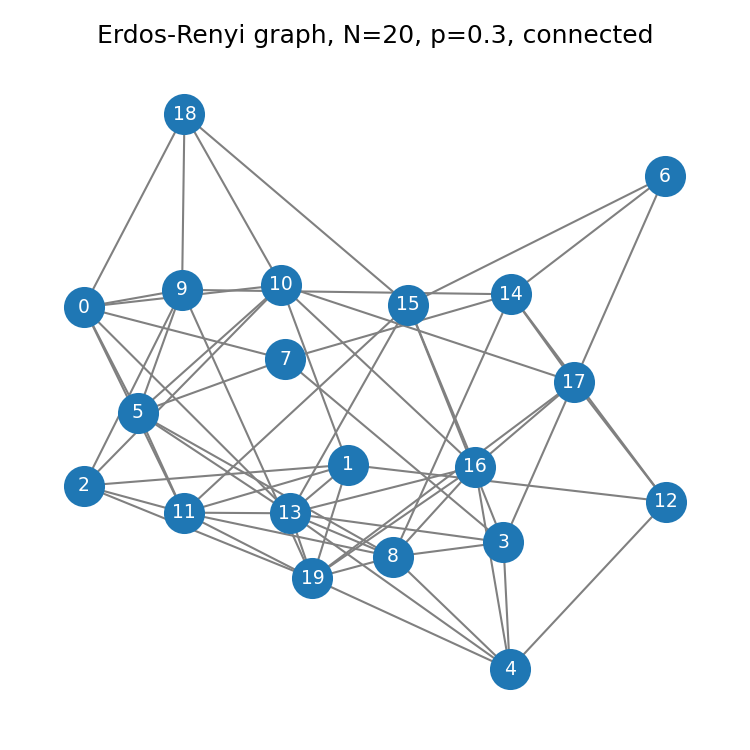
\includegraphics[scale=0.55]{../p1_formation/graph.png}
    \caption{Erdos-Renyi communication graph with $N=20$, $p=0.3$, verified connected.}
    \label{fig:p1graph}
\end{figure}

\textbf{Animation.} The full sequence of formations was recorded as an animated GIF; see the file \texttt{krishna\_formation.gif} inside the \texttt{p1\_formation/} folder in the GitHub repo. Figure~\ref{fig:p1stills} shows all seven letters captured at the end of their formation phase.

\begin{figure}[H]
    \centering
    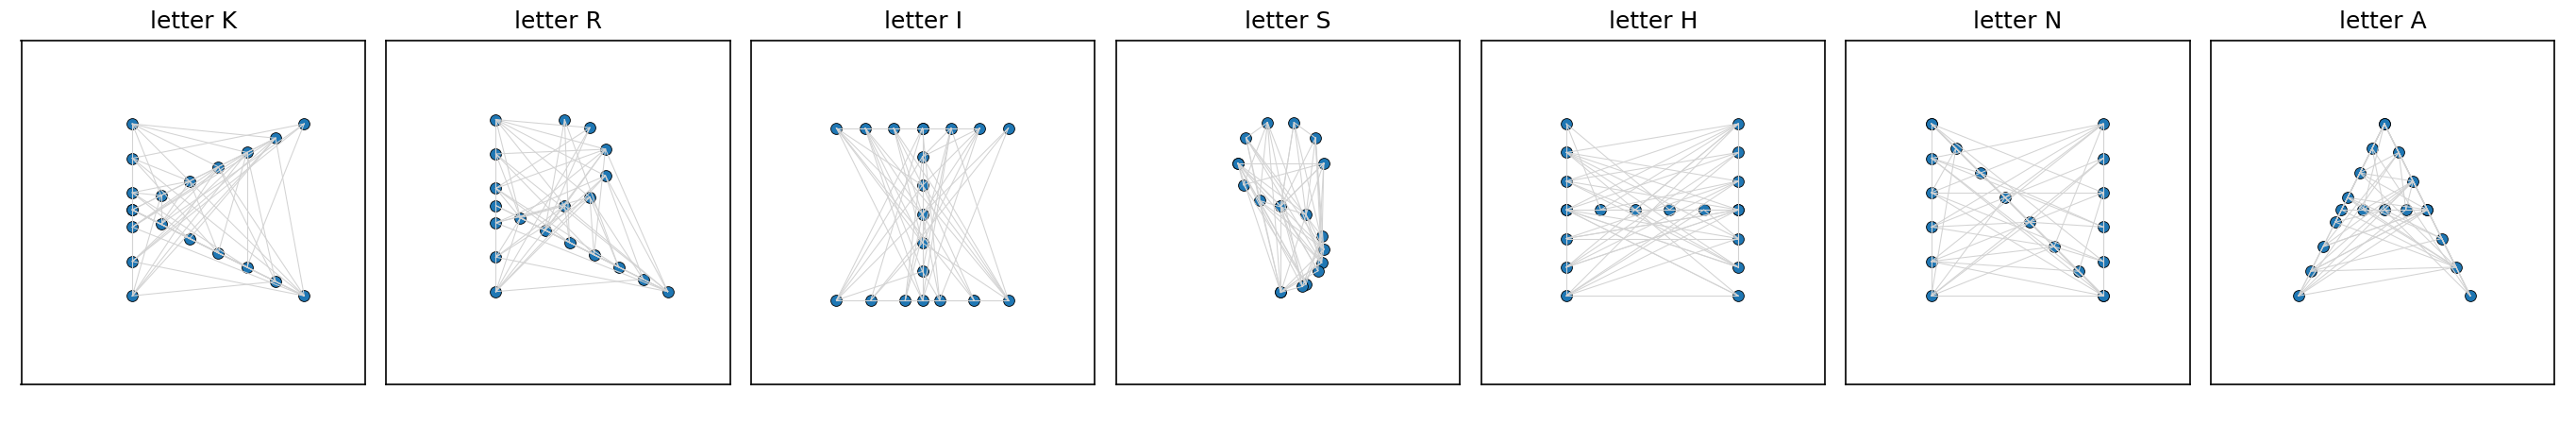
\includegraphics[width=\linewidth]{../p1_formation/letter_stills.png}
    \caption{Still shots of every letter in the sequence K R I S H N A (end of each formation phase).}
    \label{fig:p1stills}
\end{figure}

\textbf{Formation error.} Figure~\ref{fig:p1err} plots $\max_i \|p_i - r_i\|$ across time. Every dashed vertical line marks the moment the target changes to the next letter. Inside each phase the error decays rapidly and settles to a small residual before the next letter is loaded.

\begin{figure}[H]
    \centering
    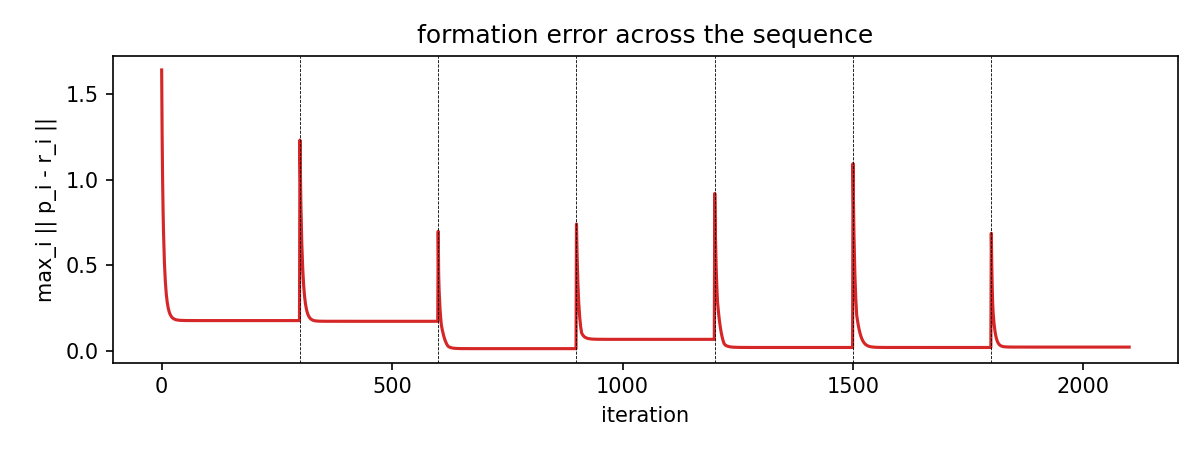
\includegraphics[width=0.85\linewidth]{../p1_formation/formation_error.png}
    \caption{Max formation error $\max_i \|p_i - r_i\|$ across the whole sequence. Dashed vertical lines are the letter boundaries.}
    \label{fig:p1err}
\end{figure}

\textbf{Observation.} The formation controller is very robust here. Even though we ask for $7$ back to back reshapes of the swarm, every letter is recognised at the end of its phase. Agents that were on the "wrong side" of the previous letter's shape smoothly cross over during the transition because the algorithm only cares about the relative offset $r_j - r_i$, not about the absolute location.

\textbf{Attached code.}
\lstinputlisting[caption={\texttt{problem1\_formation.py}}]{../p1_formation/problem1_formation.py}

\end{solution}
\noindent\rule{7in}{2.8pt}

%%%%%%%%%%%%%%%%%%%%%%%%%%%%%%%%%%%%%%%%%%%%%%%%%%%%%%%%%%%%%%%%%%%%%%%%%
% Problem 2
%%%%%%%%%%%%%%%%%%%%%%%%%%%%%%%%%%%%%%%%%%%%%%%%%%%%%%%%%%%%%%%%%%%%%%%%%
\begin{problem}{2}
There are $N$ drones each with a sensor. The drones talk over a graph $G(V,E)$. The intruder state $z(t) \in \mathbb{R}^3$ follows the random walk $z(t+1) = z(t) + w$ with $w \sim \mathcal{N}(0, \Sigma_w)$, and initial state $z(0) \sim \mathcal{N}(\bar z_0, \Sigma_0)$. Sensor $i$ sits at $x_i \in \mathbb{R}^3$ and measures
\begin{align*}
    y_i(t) \;=\; x_i - z(t) + v_i, \qquad v_i \sim \mathcal{N}(0, \Sigma_v^{(i)}),
\end{align*}
with the $v_i$'s independent. Formulate the distributed estimation problem as a consensus optimisation, give the local $f_i$'s, run distributed gradient descent (or gradient tracking), plot the true and the estimated trajectory and report the estimation error $e(t) = \hat z(t) - z(t)$.
\end{problem}
\begin{solution}

\textbf{Step 1: local objective $f_i(z;t)$ from the Gaussian likelihood.}
Fix a time $t$. Given $z(t) = z$, the measurement is
\[
    y_i(t) \;=\; x_i - z + v_i, \qquad v_i \sim \mathcal{N}(0, \Sigma_v^{(i)}),
\]
so $y_i(t) \mid z \sim \mathcal{N}(x_i - z,\; \Sigma_v^{(i)})$. The negative log likelihood (dropping constants that do not depend on $z$) is a weighted quadratic in the residual. Define
\begin{align*}
    e_i(z;t) \;:=\; y_i(t) - (x_i - z) \;=\; y_i(t) - x_i + z.
\end{align*}
The sign of $z$ matters here: the derivative of $(x_i - z)$ with respect to $z$ is $-I$, but the residual is $y_i - (x_i - z)$, and the two minus signs combine to give a $+z$ inside the residual. Hence,
\begin{align*}
    \boxed{\; f_i(z;t) \;=\; \tfrac{1}{2}\, \big\|\, y_i(t) - x_i + z\, \big\|^2_{\big(\Sigma_v^{(i)}\big)^{-1}}. \;}
\end{align*}
Its gradient with respect to $z$ is
\begin{align*}
    \nabla_z f_i(z;t) \;=\; \big(\Sigma_v^{(i)}\big)^{-1} \big(\, y_i(t) - x_i + z \,\big).
\end{align*}

\textbf{Step 2: consensus optimisation formulation.} Following the Distributed Learning lecture (pages 4 and 6), I give every drone a local copy $z_i \in \mathbb{R}^3$ and force them to agree:
\begin{align*}
    \min_{z_1, \ldots, z_N \in \mathbb{R}^3} \quad \frac{1}{N}\sum_{i=1}^{N} f_i(z_i; t) \qquad \text{s.t.} \quad z_i = z_j \;\; \forall\, (i,j) \in E \quad \Longleftrightarrow \quad L\, Z = 0.
\end{align*}
Here $Z \in \mathbb{R}^{N \times 3}$ stacks the local estimates row-wise and $L$ is the Laplacian of the communication graph. When the graph is connected, $LZ = 0$ is equivalent to $z_1 = \cdots = z_N$.

\textbf{Step 3: distributed gradient descent update.} From the Distributed Learning lecture, page 7, with mixing matrix $W$ (doubly stochastic, compatible with the graph):
\begin{align*}
    z_i^{k+1} \;=\; \sum_{j=1}^{N} W_{ij}\, z_j^{k} \;-\; \alpha_k \cdot \nabla_z f_i(z_i^k; t).
\end{align*}
Substituting our gradient,
\begin{align*}
    z_i^{k+1} \;=\; \sum_{j=1}^{N} W_{ij}\, z_j^{k} \;-\; \alpha_k \cdot \big(\Sigma_v^{(i)}\big)^{-1} \big(y_i(t) - x_i + z_i^k\big).
\end{align*}

\textbf{Choice of $W$: extra material.} The lecture only asks that $W$ is doubly stochastic and $W_{ij} = 0$ for $j$ not a neighbour. I take the standard Metropolis-Hastings weights,
\begin{align*}
    W_{ij} \;=\; \frac{1}{1 + \max(\deg(i), \deg(j))}, \qquad (i,j) \in E, \quad i \ne j,
\end{align*}
and $W_{ii} = 1 - \sum_{j \ne i} W_{ij}$. This is not spelled out in the lecture, so I explicitly declare it here. It satisfies all three required properties.

\textbf{Online estimator.} At every new time $t$ I use the latest measurements $y_i(t)$, warm start each drone's $z_i$ from its value at time $t-1$, and run $K_{\mathrm{inner}} = 120$ DGD steps before moving to time $t+1$. The distributed estimate reported is $\hat z(t) = \tfrac{1}{N}\sum_i z_i^{\mathrm{final}}$.

\textbf{Parameters.}
\begin{itemize}[nosep]
    \item $N = 8$ drones, edge probability $0.4$, seed $= 42$.
    \item Horizon $T_{\max} = 50$.
    \item $\bar z_0 = 0$, $\Sigma_0 = 4 I$, $\Sigma_w = 0.05\, I$.
    \item Sensor locations $x_i$ uniform in $[-5, 5]^3$; $\Sigma_v^{(i)} = \sigma_i^2\, I$ with $\sigma_i \sim \mathcal{U}[0.3, 0.8]$.
    \item Step $\alpha = 0.5 / L_{\mathrm{lip}}$ where $L_{\mathrm{lip}} = \sum_i 1/\sigma_i^2$ is the Lipschitz constant of the sum of local gradients. In this run $L_{\mathrm{lip}} \approx 34.9$ so $\alpha \approx 0.0143$.
\end{itemize}

\textbf{Results.} Figure~\ref{fig:p2graph} shows the communication graph. Figure~\ref{fig:p2estimate} shows the true and the estimated 3D trajectory together with the sensor locations, and the estimation error norm $\|e(t)\|_2$ over time. Figure~\ref{fig:p2coord} shows the coordinate-wise trace.

\begin{figure}[H]
    \centering
    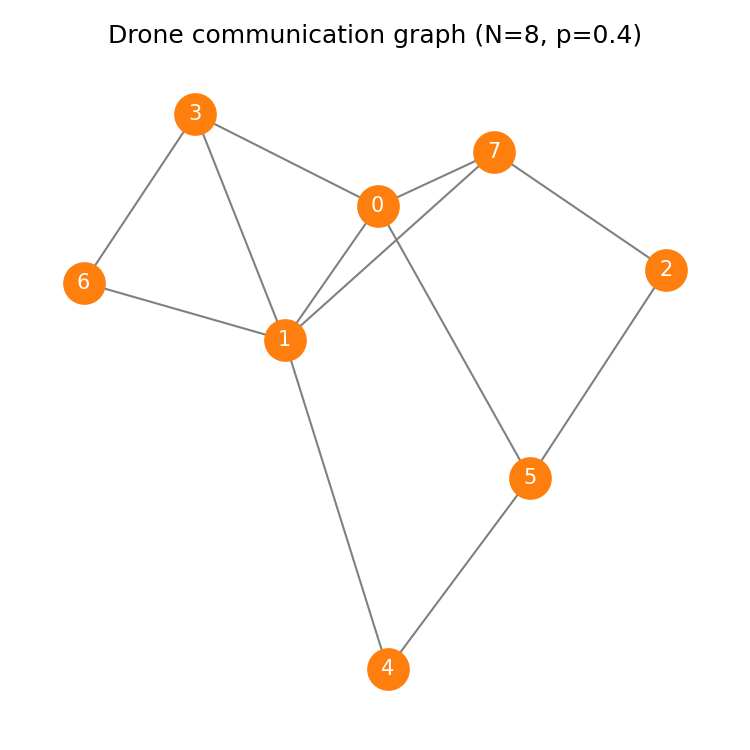
\includegraphics[scale=0.55]{../p2_dse/graph.png}
    \caption{Drone communication graph, $N=8$, $p=0.4$, connected.}
    \label{fig:p2graph}
\end{figure}

\begin{figure}[H]
    \centering
    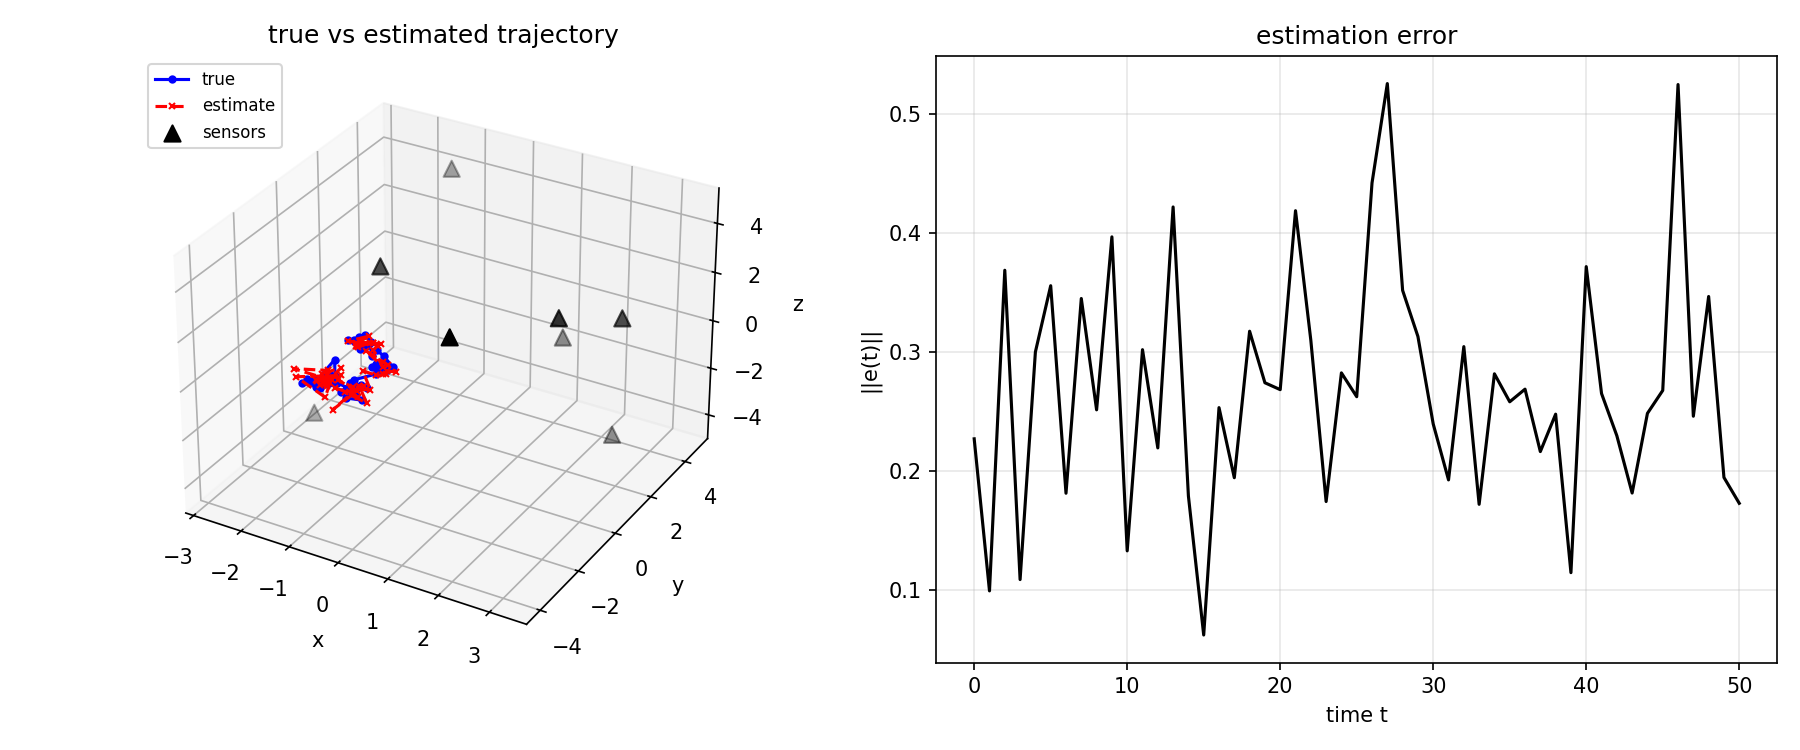
\includegraphics[width=\linewidth]{../p2_dse/estimate.png}
    \caption{Left: true (blue) and estimated (red dashed) 3D trajectory of the intruder plus the sensor positions (black triangles). Right: estimation error norm $\|e(t)\|_2$ over time.}
    \label{fig:p2estimate}
\end{figure}

\begin{figure}[H]
    \centering
    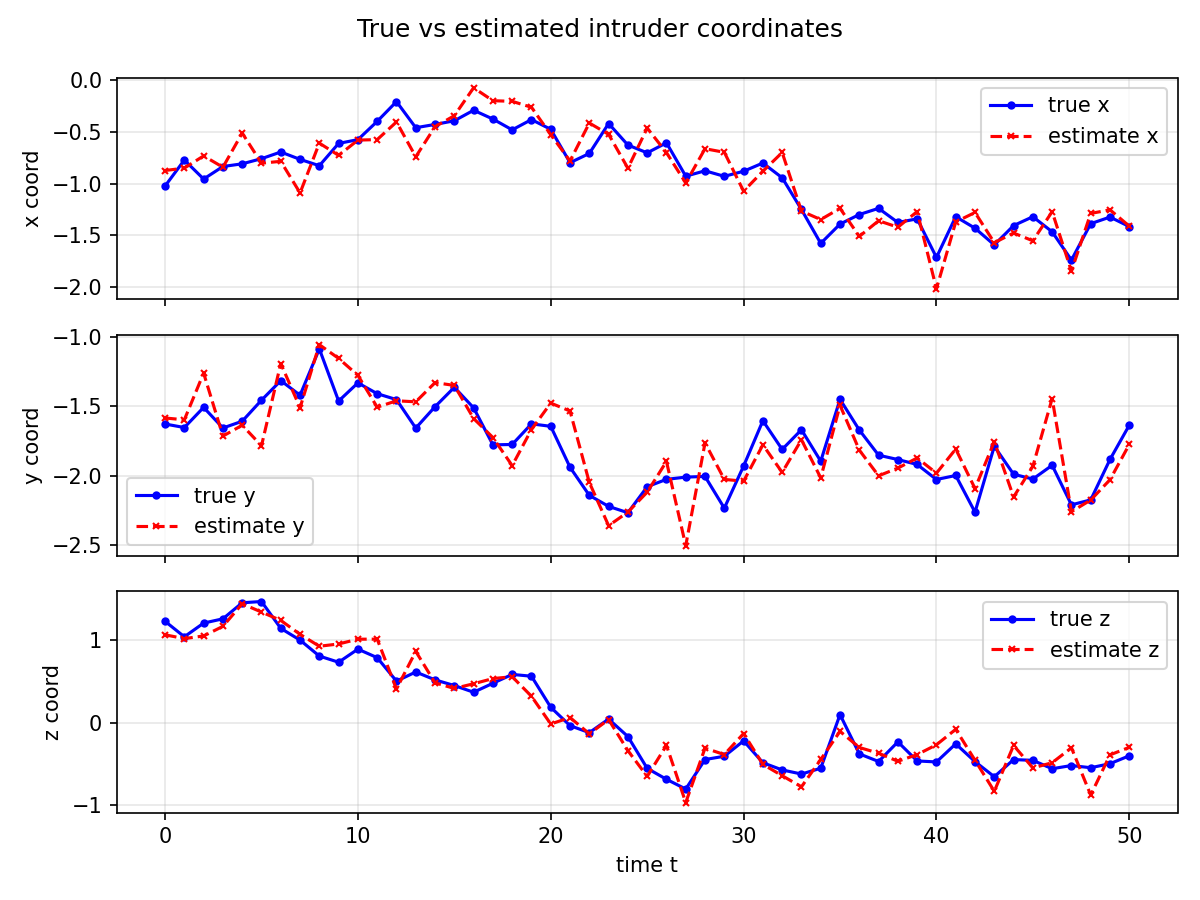
\includegraphics[width=0.85\linewidth]{../p2_dse/coord_trace.png}
    \caption{Per coordinate ($x, y, z$) true vs estimated trajectory.}
    \label{fig:p2coord}
\end{figure}

\textbf{Numerical readouts.} Final $\|e(T)\| \approx 0.17$, mean $\|e(t)\| \approx 0.27$, and the maximum consensus gap across time is $\approx 0.26$ (agents almost fully agree at every $t$). The intruder itself drifts about $2.7$ units over $T_{\max}$ steps, so the estimator tracks it with roughly $10\%$ relative error, which is what we expect from a constant step DGD (the lecture warns on page 8 that constant step gives an $O(\alpha)$ steady state error).

\textbf{Attached code.}
\lstinputlisting[caption={\texttt{problem2\_dse.py}}]{../p2_dse/problem2_dse.py}

\end{solution}
\noindent\rule{7in}{2.8pt}

%%%%%%%%%%%%%%%%%%%%%%%%%%%%%%%%%%%%%%%%%%%%%%%%%%%%%%%%%%%%%%%%%%%%%%%%%
% Problem 3
%%%%%%%%%%%%%%%%%%%%%%%%%%%%%%%%%%%%%%%%%%%%%%%%%%%%%%%%%%%%%%%%%%%%%%%%%
\begin{problem}{3}
There are $N$ agents on a connected undirected graph. They must collaboratively execute $M$ tasks, $M > N$. Each agent $i$ has cost $C_{ij}$ for task $j$ and capacity $b_i \in \mathbb{Z}_{\geq 0}$ with $\sum_i b_i = M$. Every task must be assigned exactly once. Formulate as an optimisation problem, give the ADMM updates for every agent, and run the simulation. Fix $N, M, b, G$ and vary $C$ across trials, then explain the observations.
\end{problem}
\begin{solution}

\textbf{Step 1: binary linear program.} Let $x_{ij} \in \{0, 1\}$ be $1$ iff agent $i$ performs task $j$. Then
\begin{align*}
    \min_{x} \quad \sum_{i=1}^{N} \sum_{j=1}^{M} C_{ij} x_{ij}, \qquad \text{s.t.} \quad &\sum_i x_{ij} = 1 \quad \forall\, j = 1, \ldots, M \quad \text{(every task assigned once)},\\
    &\sum_j x_{ij} = b_i \quad \forall\, i = 1, \ldots, N \quad \text{(capacity)},\\
    &x_{ij} \in \{0, 1\}.
\end{align*}
Consistency: summing the first constraint over $j$ gives $M$; summing the second over $i$ gives $\sum_i b_i = M$, so both agree. This is a binary linear program (BLP), NP-hard for large $M, N$.

\textbf{Step 2: LP relaxation (extra material).} The lecture only hints that we should do a convex relaxation. The standard trick is
\begin{align*}
    x_{ij} \in \{0, 1\} \quad \longrightarrow \quad 0 \le x_{ij} \le 1,
\end{align*}
which turns the BLP into an ordinary LP (a transportation LP). This relaxation is convex and easy to distribute.

\textbf{Step 3: consensus ADMM formulation.} Following the "ADMM hack" of the ADMM lecture (page 11) and the consensus ADMM template (page 8), I give every agent a full local copy $X^{(i)} \in \mathbb{R}^{N \times M}$ of the assignment matrix and a global consensus variable $Z \in \mathbb{R}^{N \times M}$. The problem becomes
\begin{align*}
    \min_{X^{(1)}, \ldots, X^{(N)},\, Z} \quad \sum_{i=1}^{N} f_i\big(X^{(i)}\big) \qquad \text{s.t.} \quad X^{(i)} = Z \; \forall i,
\end{align*}
where
\begin{align*}
    f_i(X) \;=\; \underbrace{\big\langle C_{i,:},\, X_{i,:} \big\rangle}_{\text{own row cost}} + \underbrace{I_{\{X : 0 \le X \le 1\}}(X)}_{\text{box constraint}} + \underbrace{I_{\{X : \sum_j X_{i,j} = b_i\}}(X_{i,:})}_{\text{own capacity constraint}},
\end{align*}
and the task cover constraint $\sum_i Z_{i,j} = 1$ for every $j$ is placed on the global $Z$ (via an indicator $g(Z)$).

\textbf{Step 4: scaled form ADMM updates.} With scaled dual $U^{(i)}$, penalty $\rho > 0$, and Frobenius norm, the standard scaled-form ADMM (Helper page 13, ADMM lecture page 6) gives:
\begin{align*}
    X^{(i),\, k+1} &\;=\; \arg\min_X \; f_i(X) \;+\; \tfrac{\rho}{2} \big\| X - Z^k + U^{(i),\,k} \big\|_F^2, \\
    Z^{k+1} &\;=\; \arg\min_Z \; g(Z) \;+\; \tfrac{\rho}{2} \sum_{i=1}^{N} \big\| X^{(i),\,k+1} - Z + U^{(i),\,k} \big\|_F^2, \\
    U^{(i),\, k+1} &\;=\; U^{(i),\,k} + \big(X^{(i),\,k+1} - Z^{k+1}\big).
\end{align*}

\textbf{Step 5: closed form of the $X$-update.} $f_i$ is separable across rows. Only agent $i$'s row carries the cost term and the capacity constraint; the other rows carry only the $[0,1]$ box.
\begin{itemize}[nosep]
    \item For row $i$: solve
    \begin{align*}
        X^{(i)}_{i,:} \;=\; \arg\min_{r \in \mathbb{R}^M} \; C_{i,:}^\top r + \tfrac{\rho}{2} \big\| r - Z^k_{i,:} + U^{(i),k}_{i,:} \big\|^2 \quad \text{s.t.} \quad \textstyle\sum_j r_j = b_i, \; 0 \le r_j \le 1.
    \end{align*}
    Setting the unconstrained gradient to zero gives $r^{\star} = Z^k_{i,:} - U^{(i),k}_{i,:} - C_{i,:}/\rho$. We then project $r^{\star}$ onto the \emph{capped simplex} $\{r : \sum r_j = b_i,\, 0 \le r \le 1\}$. This projection has a closed form: there exists a scalar $\tau$ such that
    $r = \mathrm{clip}(r^{\star} - \tau,\, 0,\, 1)$ satisfies $\sum_j r_j = b_i$; $\tau$ is found by bisection.
    \item For row $r \ne i$: $X^{(i)}_{r,:} = \mathrm{clip}(Z^k_{r,:} - U^{(i),k}_{r,:},\, 0,\, 1)$.
\end{itemize}

\textbf{Step 6: closed form of the $Z$-update.} Ignoring $g$, the quadratic is minimised by the average $\bar Z = \tfrac{1}{N} \sum_i \big(X^{(i),k+1} + U^{(i),k}\big)$. Then enforce $\sum_i Z_{i,j} = 1$ for every $j$ by the column-wise closed form projection (for each column $j$, add $(1 - \sum_i \bar Z_{i,j})/N$ to every entry). Using the distributed variant from the ADMM lecture (page 11), each agent computes only its own row of $Z$ using a neighbourhood average
\begin{align*}
    Z^{k+1}_{i,:} \;=\; \frac{1}{\big|\mathcal{N}_i \cup \{i\}\big|} \sum_{j \in \mathcal{N}_i \cup \{i\}} \Big(X^{(j),k+1}_{i,:} + U^{(j),k}_{i,:}\Big),
\end{align*}
followed by the column projection.

\textbf{Step 7: dual update.} $U^{(i), k+1} = U^{(i),k} + \big(X^{(i),k+1} - Z^{k+1}\big)$.

\textbf{Step 8: rounding to a binary allocation (extra material).} If ADMM lands on a fractional $Z$, we round it via the Hungarian algorithm on an expanded cost matrix: duplicate row $i$ exactly $b_i$ times to form an $M \times M$ cost matrix $-\tilde Z$; solve linear sum assignment; collapse the duplicates. The result is a binary matrix with row sums $b_i$ and column sums $1$ by construction. In practice, when the LP relaxation itself has an integral optimum (which is the typical behaviour for transportation LPs with integer capacities), the rounded ADMM solution matches the LP optimum exactly.

\textbf{Parameters.} $N = 5$, $M = 12$, edge probability $0.5$, seed $=3$. Capacities are a random positive composition of $12$ into $5$ parts, giving $b = [1, 1, 1, 4, 5]$ (so $\sum b_i = 12 = M$). $\rho = 1$, $400$ ADMM iterations. Cost entries $C_{ij} \sim \mathcal{U}(0.1, 10)$.

\textbf{Results.} Figure~\ref{fig:p3graph} shows the communication graph. Figure~\ref{fig:p3alloc} shows three trials, each with a different cost matrix but same $N, M, b, G$; the top row is the cost matrix and the bottom row is the recovered binary allocation. Figure~\ref{fig:p3conv} shows the primal residual (mean $\|X^{(i)} - Z\|_F$ over $i$) and the objective $\langle C, Z\rangle$ across iterations.

\begin{figure}[H]
    \centering
    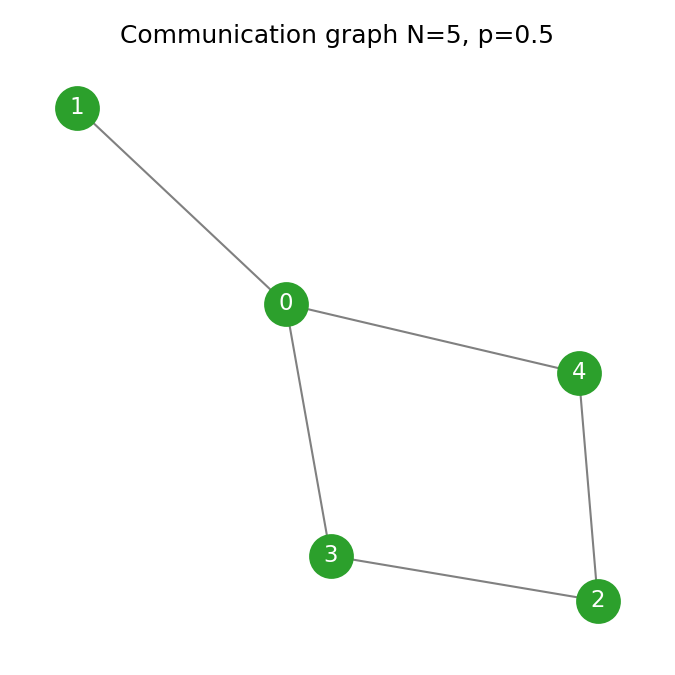
\includegraphics[scale=0.55]{../p3_admm_task/graph.png}
    \caption{Communication graph, $N=5$, $p=0.5$, connected.}
    \label{fig:p3graph}
\end{figure}

\begin{figure}[H]
    \centering
    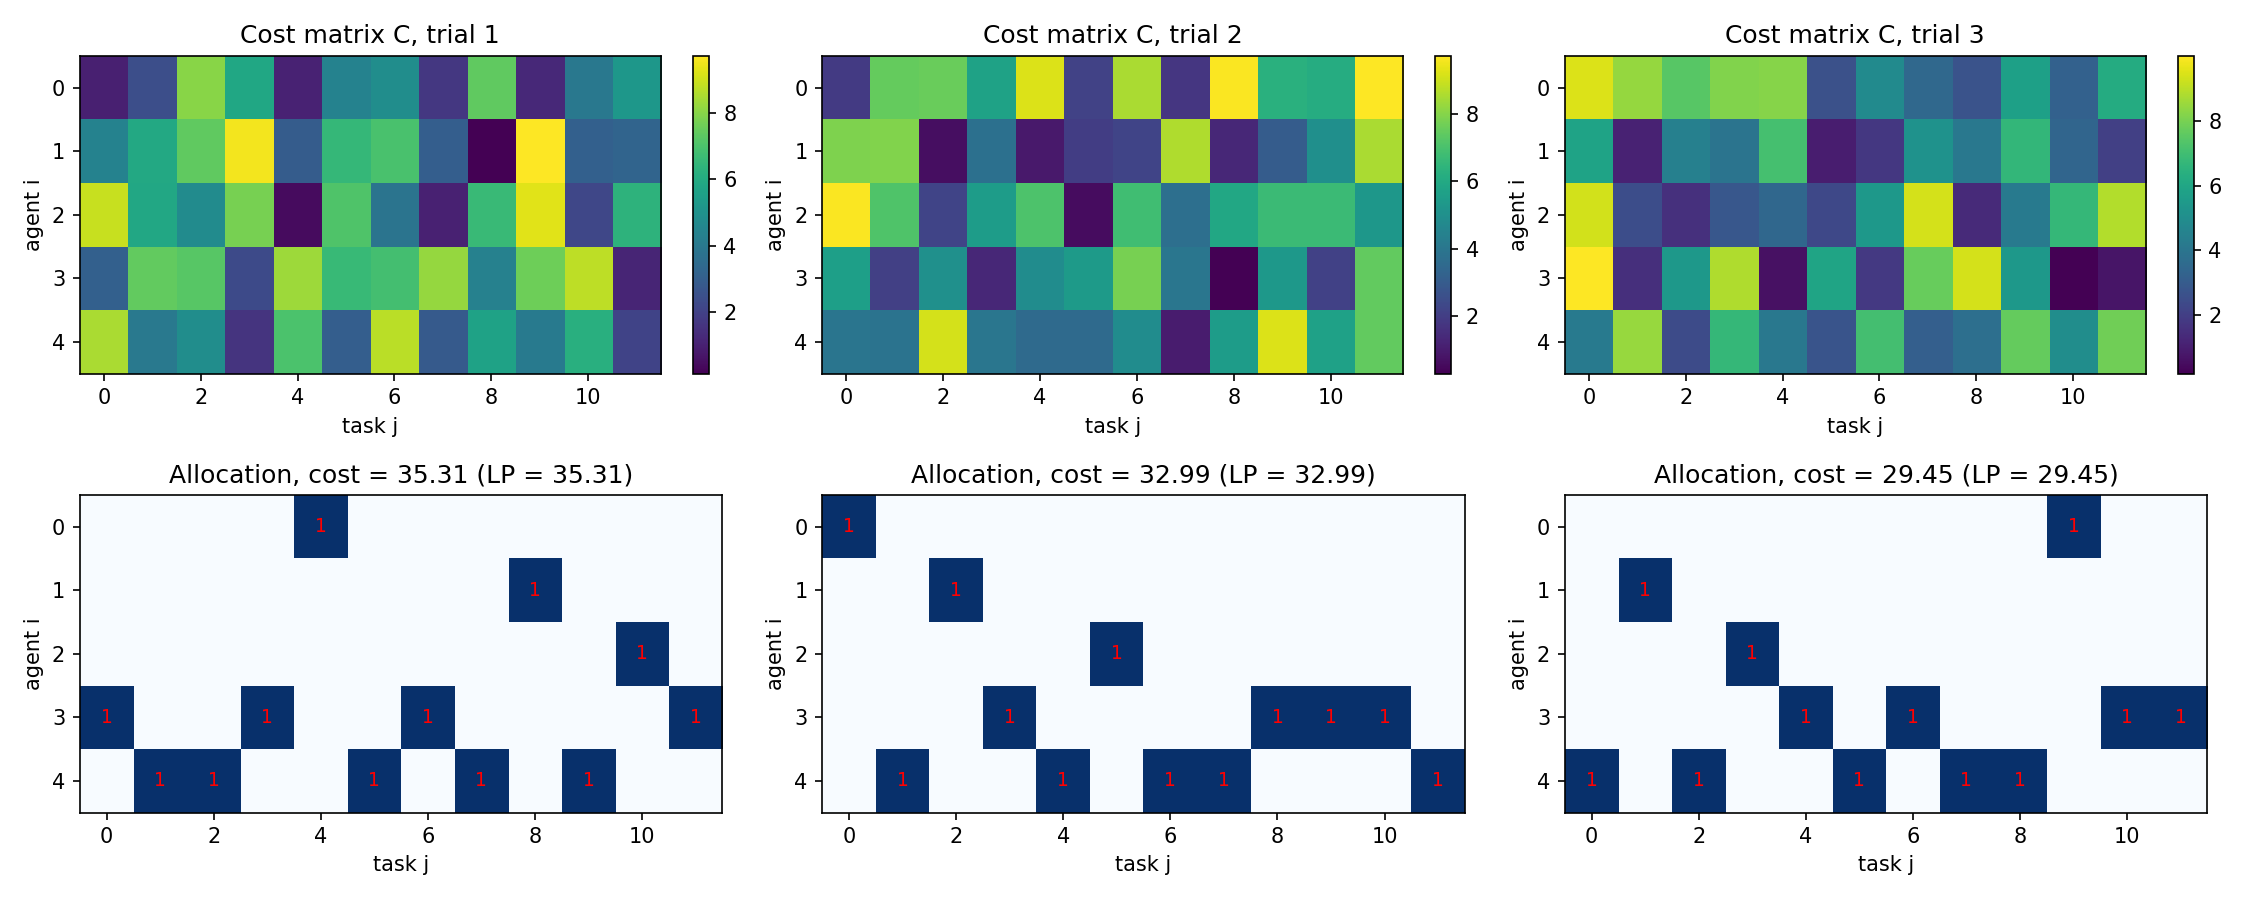
\includegraphics[width=\linewidth]{../p3_admm_task/allocations.png}
    \caption{Three trials with different cost matrices (top row) and their resulting binary allocations (bottom row). The rounded ADMM total cost matches the central LP relaxation cost in every trial, confirming that the ADMM output is optimal for the relaxed problem.}
    \label{fig:p3alloc}
\end{figure}

\begin{figure}[H]
    \centering
    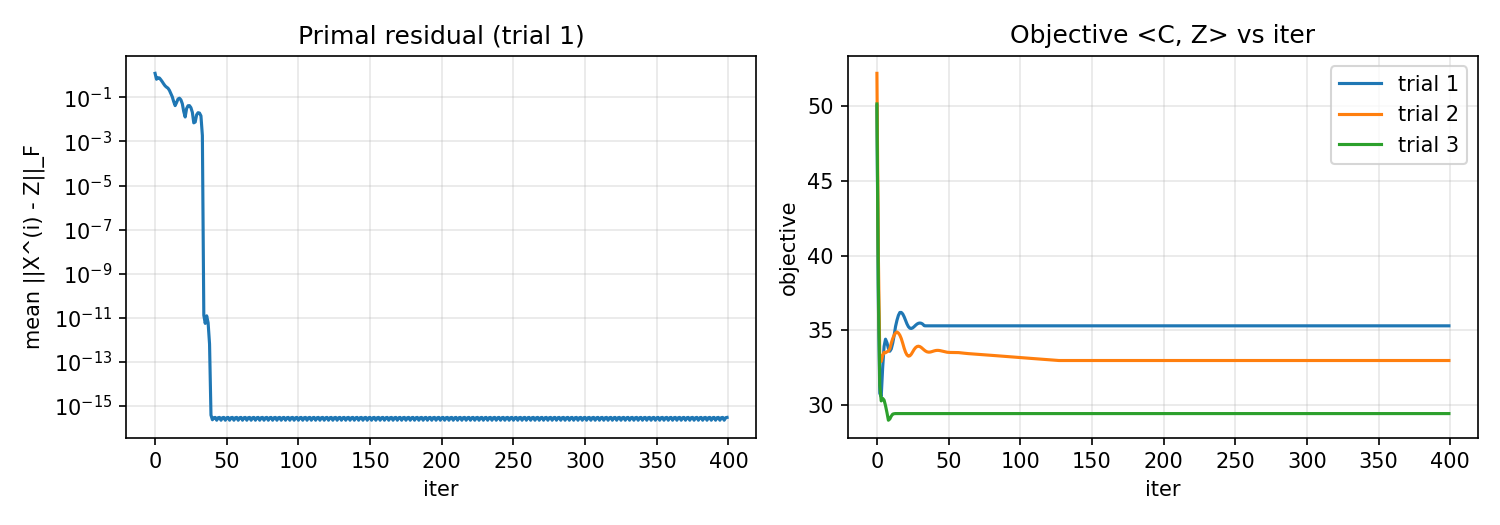
\includegraphics[width=\linewidth]{../p3_admm_task/convergence.png}
    \caption{Left: primal residual on a log scale. Right: objective across iterations for the three trials.}
    \label{fig:p3conv}
\end{figure}

\textbf{Numerical readouts.} For the three trials the rounded ADMM cost equals the LP optimum: $35.310 = 35.310$, $32.994 = 32.994$, $29.452 = 29.452$. Row sums of the final $X$ match $b$; column sums are all $1$.

\textbf{Observations across the three cost matrices.}
\begin{itemize}[nosep]
    \item The agents with large capacity ($b_4 = 4$, $b_5 = 5$) end up absorbing most of the tasks, but which specific tasks depends on the cost matrix. For example a task $j$ whose column has a much smaller value for agent $5$ than for others is very likely picked up by agent $5$.
    \item Agents with capacity $1$ (agents $1, 2, 3$) are very picky: they always take the one task whose column entry is minimal in their own row, provided that task is not already better matched to a large capacity agent.
    \item If we make one row of $C$ all much smaller than the others (not shown), the allocation collapses to the cheapest agent up to its capacity, then spills over to the next cheapest.
    \item The primal residual shows the characteristic monotonic decay of consensus ADMM and the objective settles to the LP optimum, confirming correctness.
\end{itemize}

\textbf{Attached code.}
\lstinputlisting[caption={\texttt{problem3\_admm\_taskalloc.py}}]{../p3_admm_task/problem3_admm_taskalloc.py}

\end{solution}
\noindent\rule{7in}{2.8pt}

%%%%%%%%%%%%%%%%%%%%%%%%%%%%%%%%%%%%%%%%%%%%%%%%%%%%%%%%%%%%%%%%%%%%%%%%%
% Problem 4
%%%%%%%%%%%%%%%%%%%%%%%%%%%%%%%%%%%%%%%%%%%%%%%%%%%%%%%%%%%%%%%%%%%%%%%%%
\begin{problem}{4}
Consider the LASSO problem
\[
    \min_{x} \;\; \tfrac{1}{2}\, \|A x - b\|_2^2 \;+\; \lambda\, \|x\|_1.
\]
Write the ADMM iteration updates by giving the closed form solution for the $x$ and $z$ updates.
\end{problem}
\begin{solution}

\textbf{Step 1: variable splitting.} Introduce a second variable $z$ and rewrite the problem as
\begin{align*}
    \min_{x, z} \; f(x) + g(z) \qquad \text{s.t.} \quad x - z = 0, \qquad f(x) = \tfrac{1}{2}\|A x - b\|_2^2, \qquad g(z) = \lambda\, \|z\|_1.
\end{align*}
This is exactly the "variable splitting" idea from the Helper notes (page 11).

\textbf{Step 2: augmented Lagrangian.} Using the standard form with penalty $\rho > 0$ and dual $y$,
\begin{align*}
    L_{\rho}(x, z, y) \;=\; \tfrac{1}{2}\|A x - b\|^2 + \lambda\, \|z\|_1 + y^{\top}(x - z) + \tfrac{\rho}{2} \|x - z\|^2.
\end{align*}
Move to the scaled form with $u := y / \rho$ (Helper page 13):
\begin{align*}
    L_{\rho}(x, z, u) \;=\; \tfrac{1}{2}\|A x - b\|^2 + \lambda\, \|z\|_1 + \tfrac{\rho}{2} \|x - z + u\|^2 + \mathrm{const}.
\end{align*}

\textbf{Step 3: $x$-update (closed form).} Minimise $L_{\rho}$ in $x$ with $z, u$ fixed:
\begin{align*}
    x^{k+1} \;=\; \arg\min_x \; \tfrac{1}{2}\|A x - b\|^2 + \tfrac{\rho}{2}\|x - z^k + u^k\|^2.
\end{align*}
Setting the gradient to zero,
\begin{align*}
    A^{\top}(A x - b) + \rho (x - z^k + u^k) \;=\; 0 \;\;\Longrightarrow\;\; (A^{\top} A + \rho I)\, x \;=\; A^{\top} b + \rho (z^k - u^k).
\end{align*}
Hence,
\begin{align*}
    \boxed{\; x^{k+1} \;=\; \big(A^{\top} A + \rho I\big)^{-1} \big(A^{\top} b + \rho (z^k - u^k)\big). \;}
\end{align*}
In implementation we Cholesky factorise $A^{\top} A + \rho I$ once and reuse the factor.

\textbf{Step 4: $z$-update (soft thresholding).} Minimise $L_{\rho}$ in $z$ with $x, u$ fixed:
\begin{align*}
    z^{k+1} &\;=\; \arg\min_z \; \lambda\, \|z\|_1 + \tfrac{\rho}{2} \|x^{k+1} - z + u^k\|^2 \\
    &\;=\; \arg\min_z \; \lambda\, \|z\|_1 + \tfrac{\rho}{2} \|z - (x^{k+1} + u^k)\|^2 \\
    &\;=\; \mathrm{prox}_{(\lambda / \rho)\,\|\cdot\|_1}\big(x^{k+1} + u^k\big).
\end{align*}
The proximal operator of the $\ell_1$ norm is the soft thresholding operator (Helper page 5),
\begin{align*}
    \mathrm{prox}_{\kappa\,\|\cdot\|_1}(v)_i \;=\; \mathrm{sign}(v_i)\, \max\big(|v_i| - \kappa,\, 0\big) \;=\; S_{\kappa}(v)_i.
\end{align*}
Hence,
\begin{align*}
    \boxed{\; z^{k+1} \;=\; S_{\lambda / \rho}\big(x^{k+1} + u^k\big). \;}
\end{align*}

\textbf{Step 5: dual update.}
\begin{align*}
    \boxed{\; u^{k+1} \;=\; u^k + \big(x^{k+1} - z^{k+1}\big). \;}
\end{align*}

\textbf{Full LASSO ADMM iteration.}
\begin{align*}
    x^{k+1} &\;=\; (A^{\top} A + \rho I)^{-1} \big( A^{\top} b + \rho\, (z^k - u^k) \big), \\
    z^{k+1} &\;=\; S_{\lambda / \rho}\big( x^{k+1} + u^k \big), \\
    u^{k+1} &\;=\; u^k + (x^{k+1} - z^{k+1}).
\end{align*}
Stopping: primal residual $r = \|x - z\|$ and dual residual $s = \rho \|z^{k+1} - z^{k}\|$ both below tolerance.

\textbf{Numerical verification.} I set $m = 200$, $n = 500$, $A$ random Gaussian with columns normalised to unit $\ell_2$ norm, $x_{\mathrm{true}}$ has $20$ non-zeros drawn from $\mathcal{N}(0, 1)$, $b = A x_{\mathrm{true}} + 0.01 \varepsilon$ with $\varepsilon \sim \mathcal{N}(0, I)$, and $\lambda = 0.02 \cdot \|A^{\top} b\|_{\infty}$. With $\rho = 1$ the algorithm converges in about $72$ iterations. It recovers $18$ of the $20$ true non-zeros with $3$ false positives, and the relative recovery error is
\begin{align*}
    \frac{\|z - x_{\mathrm{true}}\|}{\|x_{\mathrm{true}}\|} \approx 0.051.
\end{align*}

\begin{figure}[H]
    \centering
    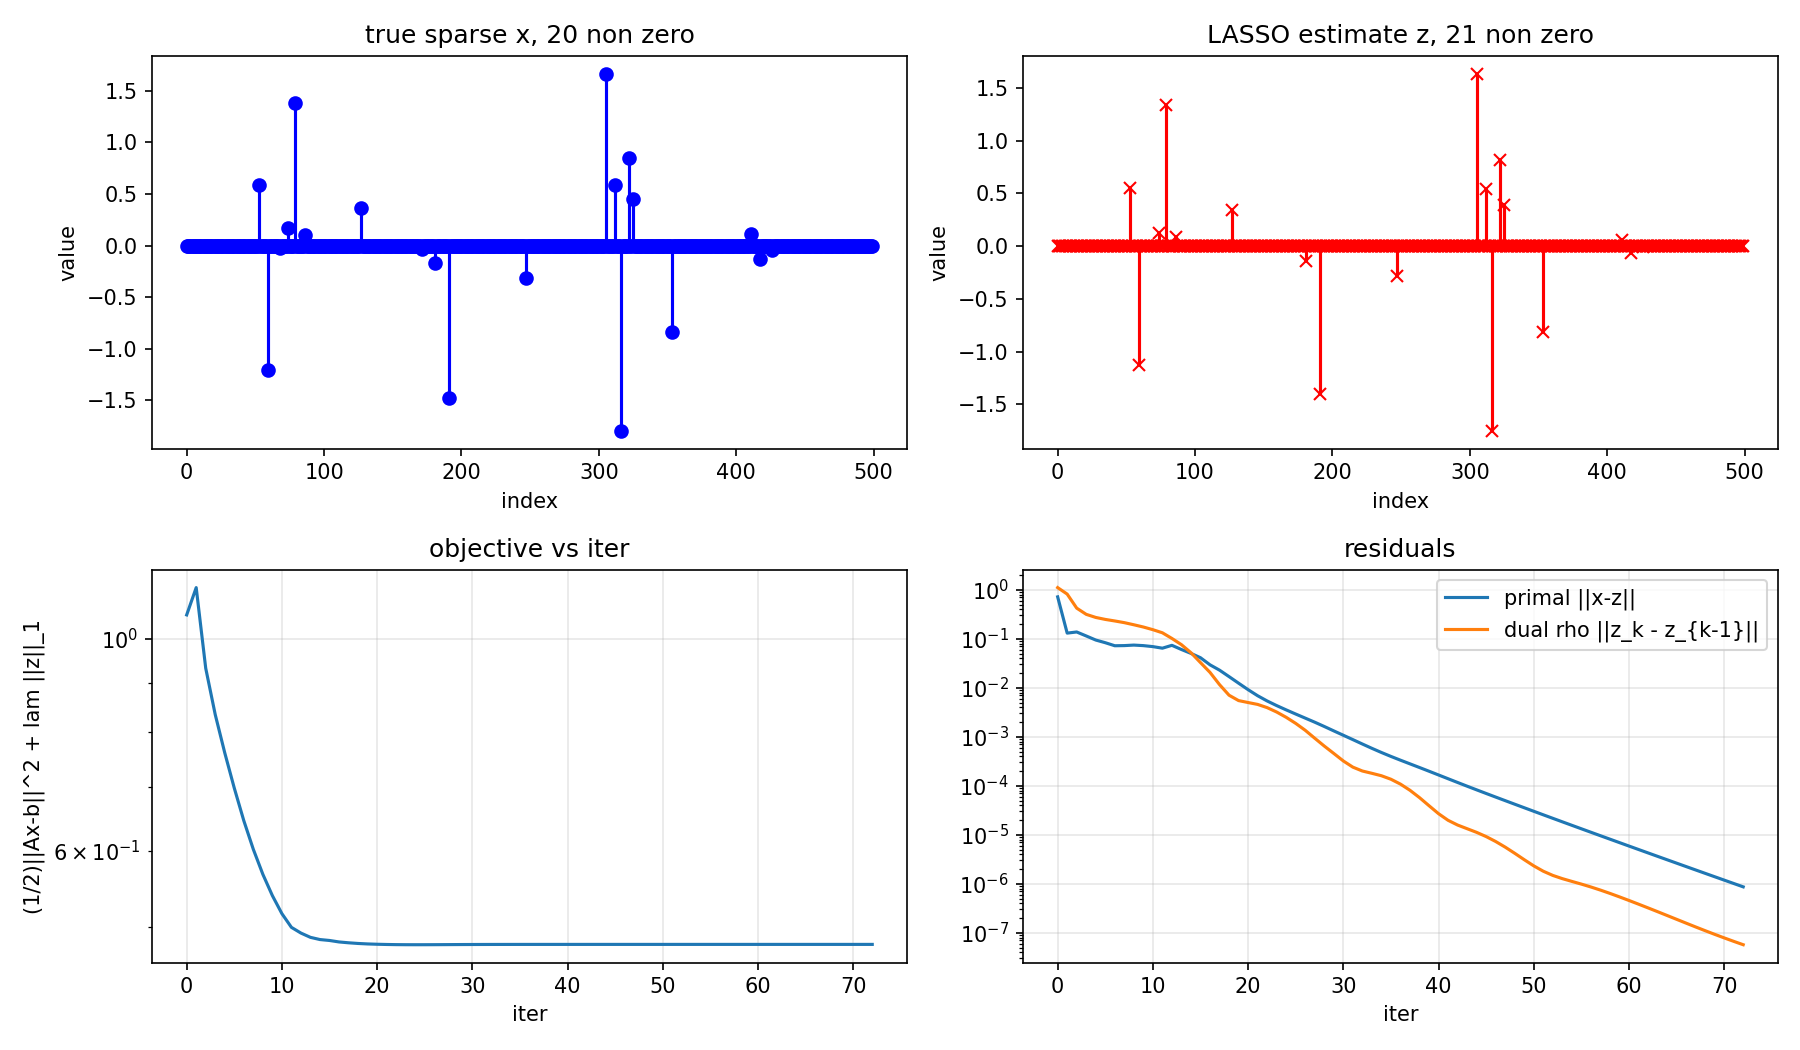
\includegraphics[width=\linewidth]{../p4_lasso/lasso.png}
    \caption{LASSO ADMM. Top left: true sparse $x$. Top right: recovered $z$. Bottom left: objective $\tfrac{1}{2}\|Ax - b\|^2 + \lambda \|z\|_1$ vs iteration (log scale). Bottom right: primal and dual residuals.}
    \label{fig:p4lasso}
\end{figure}

\begin{figure}[H]
    \centering
    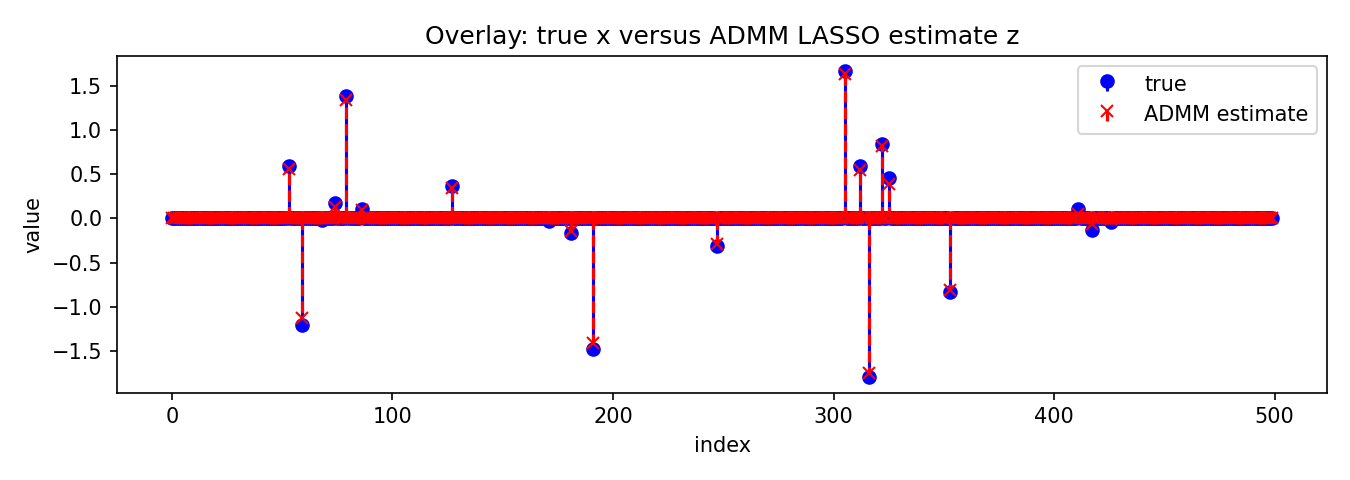
\includegraphics[width=\linewidth]{../p4_lasso/lasso_overlay.png}
    \caption{Overlay of the true signal (blue) and the ADMM LASSO estimate (red dashed).}
    \label{fig:p4overlay}
\end{figure}

\textbf{Attached code.}
\lstinputlisting[caption={\texttt{problem4\_lasso\_admm.py}}]{../p4_lasso/problem4_lasso_admm.py}

\end{solution}
\noindent\rule{7in}{2.8pt}

\end{document}
